\documentclass[
  shownotes,
  xcolor={svgnames},
  hyperref={colorlinks,citecolor=DarkBlue,linkcolor=DarkRed,urlcolor=DarkBlue}
  ]{beamer}
\usepackage{animate}
\usepackage{amsmath}
\usepackage{amsfonts}
\usepackage{amssymb}
\usepackage{pifont}
\usepackage{mathpazo}
%\usepackage{xcolor}
\usepackage{multimedia}
\usepackage{fancybox}
\usepackage[para]{threeparttable}
\usepackage{multirow}
\setcounter{MaxMatrixCols}{30}
\usepackage{subcaption}
\usepackage{graphicx}
\usepackage{lscape}
\usepackage[compatibility=false,font=small]{caption}
\usepackage{booktabs}
\usepackage{ragged2e}
\usepackage{chronosys}
\usepackage{appendixnumberbeamer}
\usepackage{animate}
\setbeamertemplate{caption}[numbered]
\usepackage{color}
%\usepackage{times}
\usepackage{tikz}
\usepackage{comment} %to comment
%% BibTeX settings
\usepackage{natbib}
\bibliographystyle{apalike}
\bibpunct{(}{)}{,}{a}{,}{,}
\setbeamertemplate{bibliography item}{[\theenumiv]}

% Defines columns for bespoke tables
\usepackage{array}
\newcolumntype{L}[1]{>{\raggedright\let\newline\\\arraybackslash\hspace{0pt}}m{#1}}
\newcolumntype{C}[1]{>{\centering\let\newline\\\arraybackslash\hspace{0pt}}m{#1}}
\newcolumntype{R}[1]{>{\raggedleft\let\newline\\\arraybackslash\hspace{0pt}}m{#1}}


\usepackage{xfrac}


\usepackage{multicol}
\setlength{\columnsep}{0.5cm}

% Theme and colors
\usetheme{Boadilla}

% I use steel blue and a custom color palette. This defines it.
\definecolor{andesred}{HTML}{af2433}

% Other options
\providecommand{\U}[1]{\protect\rule{.1in}{.1in}}
\usefonttheme{serif}
\setbeamertemplate{itemize items}[default]
\setbeamertemplate{enumerate items}[square]
\setbeamertemplate{section in toc}[circle]

\makeatletter

\definecolor{mybackground}{HTML}{82CAFA}
\definecolor{myforeground}{HTML}{0000A0}

\setbeamercolor{normal text}{fg=black,bg=white}
\setbeamercolor{alerted text}{fg=red}
\setbeamercolor{example text}{fg=black}

\setbeamercolor{background canvas}{fg=myforeground, bg=white}
\setbeamercolor{background}{fg=myforeground, bg=mybackground}

\setbeamercolor{palette primary}{fg=black, bg=gray!30!white}
\setbeamercolor{palette secondary}{fg=black, bg=gray!20!white}
\setbeamercolor{palette tertiary}{fg=white, bg=andesred}

\setbeamercolor{frametitle}{fg=andesred}
\setbeamercolor{title}{fg=andesred}
\setbeamercolor{block title}{fg=andesred}
\setbeamercolor{itemize item}{fg=andesred}
\setbeamercolor{itemize subitem}{fg=andesred}
\setbeamercolor{itemize subsubitem}{fg=andesred}
\setbeamercolor{enumerate item}{fg=andesred}
\setbeamercolor{item projected}{bg=gray!30!white,fg=andesred}
\setbeamercolor{enumerate subitem}{fg=andesred}
\setbeamercolor{section number projected}{bg=gray!30!white,fg=andesred}
\setbeamercolor{section in toc}{fg=andesred}
\setbeamercolor{caption name}{fg=andesred}
\setbeamercolor{button}{bg=gray!30!white,fg=andesred}


\usepackage{fancyvrb}
\newcommand{\VerbBar}{|}
\newcommand{\VERB}{\Verb[commandchars=\\\{\}]}
\DefineVerbatimEnvironment{Highlighting}{Verbatim}{commandchars=\\\{\}}
% Add ',fontsize=\small' for more characters per line
\usepackage{framed}
\definecolor{shadecolor}{RGB}{248,248,248}
\newenvironment{Shaded}{\begin{snugshade}}{\end{snugshade}}
\newcommand{\AlertTok}[1]{\textcolor[rgb]{0.94,0.16,0.16}{#1}}
\newcommand{\AnnotationTok}[1]{\textcolor[rgb]{0.56,0.35,0.01}{\textbf{\textit{#1}}}}
\newcommand{\AttributeTok}[1]{\textcolor[rgb]{0.77,0.63,0.00}{#1}}
\newcommand{\BaseNTok}[1]{\textcolor[rgb]{0.00,0.00,0.81}{#1}}
\newcommand{\BuiltInTok}[1]{#1}
\newcommand{\CharTok}[1]{\textcolor[rgb]{0.31,0.60,0.02}{#1}}
\newcommand{\CommentTok}[1]{\textcolor[rgb]{0.56,0.35,0.01}{\textit{#1}}}
\newcommand{\CommentVarTok}[1]{\textcolor[rgb]{0.56,0.35,0.01}{\textbf{\textit{#1}}}}
\newcommand{\ConstantTok}[1]{\textcolor[rgb]{0.00,0.00,0.00}{#1}}
\newcommand{\ControlFlowTok}[1]{\textcolor[rgb]{0.13,0.29,0.53}{\textbf{#1}}}
\newcommand{\DataTypeTok}[1]{\textcolor[rgb]{0.13,0.29,0.53}{#1}}
\newcommand{\DecValTok}[1]{\textcolor[rgb]{0.00,0.00,0.81}{#1}}
\newcommand{\DocumentationTok}[1]{\textcolor[rgb]{0.56,0.35,0.01}{\textbf{\textit{#1}}}}
\newcommand{\ErrorTok}[1]{\textcolor[rgb]{0.64,0.00,0.00}{\textbf{#1}}}
\newcommand{\ExtensionTok}[1]{#1}
\newcommand{\FloatTok}[1]{\textcolor[rgb]{0.00,0.00,0.81}{#1}}
\newcommand{\FunctionTok}[1]{\textcolor[rgb]{0.00,0.00,0.00}{#1}}
\newcommand{\ImportTok}[1]{#1}
\newcommand{\InformationTok}[1]{\textcolor[rgb]{0.56,0.35,0.01}{\textbf{\textit{#1}}}}
\newcommand{\KeywordTok}[1]{\textcolor[rgb]{0.13,0.29,0.53}{\textbf{#1}}}
\newcommand{\NormalTok}[1]{#1}
\newcommand{\OperatorTok}[1]{\textcolor[rgb]{0.81,0.36,0.00}{\textbf{#1}}}
\newcommand{\OtherTok}[1]{\textcolor[rgb]{0.56,0.35,0.01}{#1}}
\newcommand{\PreprocessorTok}[1]{\textcolor[rgb]{0.56,0.35,0.01}{\textit{#1}}}
\newcommand{\RegionMarkerTok}[1]{#1}
\newcommand{\SpecialCharTok}[1]{\textcolor[rgb]{0.00,0.00,0.00}{#1}}
\newcommand{\SpecialStringTok}[1]{\textcolor[rgb]{0.31,0.60,0.02}{#1}}
\newcommand{\StringTok}[1]{\textcolor[rgb]{0.31,0.60,0.02}{#1}}
\newcommand{\VariableTok}[1]{\textcolor[rgb]{0.00,0.00,0.00}{#1}}
\newcommand{\VerbatimStringTok}[1]{\textcolor[rgb]{0.31,0.60,0.02}{#1}}
\newcommand{\WarningTok}[1]{\textcolor[rgb]{0.56,0.35,0.01}{\textbf{\textit{#1}}}}
\usepackage{graphicx}
\makeatletter

\makeatother






%%%%%%%%%%%%%%% BEGINS DOCUMENT %%%%%%%%%%%%%%%%%%

\begin{document}

\title[Lecture 5]{Lecture 5: Intro to Big Data, \\ OLS Numerical Properties}
\subtitle{Big Data and Machine Learning for Applied Economics \\ Econ 4676}
\date{\today}

\author[Sarmiento-Barbieri]{Ignacio Sarmiento-Barbieri}
\institute[Uniandes]{Universidad de los Andes}


\begin{frame}[noframenumbering]
\maketitle
\end{frame}


%----------------------------------------------------------------------%

\begin{frame}
\frametitle{Recap}

\begin{itemize} 

    \item Prediction vs Estimation
    \bigskip
    \item Train and Test Samples
    \bigskip
    \item Linear Regression 
    \bigskip
    \item Example in \texttt{R}
    \bigskip
    \item Machine Learning $\rightarrow$ build robust predictions from complex data
    \bigskip
    \item Problem Set 1 is up
\end{itemize}
\end{frame}



%----------------------------------------------------------------------%
\begin{frame}
\frametitle{Agenda}

\tableofcontents


\end{frame}

%----------------------------------------------------------------------%
\section{Motivation}
%----------------------------------------------------------------------%
\begin{frame}
\frametitle{Motivation}

\begin{itemize}
  \item {\it Big Data} has its origin in computer engineering
  \begin{itemize}
    \item Data so large that cannot be loaded into memory or even stored on a single machine.
    \item We need tools, distributed algorithms, that can compute data summaries across multiple independent machines. 
    \item The bigness comes from {\it ``n''}
  \end{itemize}
  \bigskip
  \item But volume is only a part of the story
  \bigskip
  \item This is data of high complexity: anarchic and spontaneous
  \bigskip
  \item They are the by product of an action: pay with a credit card, browse the web, tweet, etc...



\end{itemize}
\end{frame}

%----------------------------------------------------------------------%
\begin{frame}
\frametitle{Motivation}

\begin{itemize}
  \item We are going to start exploring tools to
  \begin{itemize}
    \item Handle 
    \medskip
    \item Acquire
    \medskip
    \item Model 
   \end{itemize}
   \bigskip
  \item Today we move in familiar waters
  \bigskip
  \item We are going to explore some properties of linear regression to  handle {\it ``Big Data''}

\end{itemize}
\end{frame}


%----------------------------------------------------------------------%
\begin{frame}
\frametitle{Motivation}

\begin{itemize}
\item Model $f(x)$ we begin in familiar waters:

\begin{align}
y = X \beta +u
\end{align}

where 
\begin{itemize}
  \item y is the dependent variable, a vector $n \times 1$ 
  \item X is a matrix of $k-1$ explanatory variables and an intercept, so its dimension is $n \times k$ 
  \item $\beta$ is a vector of coefficients $k \times 1$ 
  \item $u$ is the error term, a vector $n \times 1$ 
\end{itemize}

\bigskip
\item How do we estimate $\beta$?

\end{itemize}
\end{frame}


%----------------------------------------------------------------------%
\begin{frame}
\frametitle{OLS}
How do we estimate $\beta$?

\begin{itemize}
  \item Least squares $\rightarrow$ most widely used
  \item Consider the following loss function, where we minimize the sum of square residuals
\begin{align}
  SSR(\tilde \beta) \equiv \sum_{i=1}^n \tilde e_i^2 = \tilde e' \tilde e  = (Y-X \tilde \beta)'(Y-X \tilde \beta)
\end{align}
  \begin{itemize}
    \footnotesize
  \item $SSR(\tilde \beta)$ is the aggregation of squared errors if we choose $\tilde \beta$ as an estimator.
  \end{itemize}  

  \bigskip

    \item The {\bf least squares estimator $\hat \beta$} will be

    \begin{align}
      \hat \beta = \underset{\tilde \beta}{argmin}\, SSR(\tilde \beta)
    \end{align}

\end{itemize}

\end{frame}

%----------------------------------------------------------------------%

\begin{frame}
\frametitle{OLS}

\begin{align}
  SSR(\tilde \beta) &= \tilde e' \tilde e  \\
  &= (Y-X \tilde \beta)'(Y-X \tilde \beta)
\end{align}

FOC are

\begin{align}
 \frac{\partial \tilde{e}' \tilde{e}}{\partial \tilde \beta} &=0   \\
 \frac{\partial \tilde{e}' \tilde{e}}{\partial \tilde \beta}  =&-2X'Y + 2X'X \tilde\beta =0
\end{align}

\end{frame}

%----------------------------------------------------------------------%

\begin{frame}
\frametitle{OLS}

Let $\hat \beta$ be the solution.Then $\hat \beta$ satisfies the following normal equation

\begin{align}
X'X\hat \beta=X'y
\end{align}

If the inverse of $X'X$ exists, then

\begin{align}
\hat \beta=(X'X)^{-1}X'y
\end{align}


\end{frame}


%----------------------------------------------------------------------%
\section{Statistical Properties}
%----------------------------------------------------------------------%
\begin{frame}
\frametitle{Statistical Properties}

Under certain assumptions {\tiny HW Review the Assumption from Econometrics}
\bigskip
\begin{itemize}
  \item Small Sample
  \begin{itemize}
    \item Unbiased: $E(\hat \beta) = \beta$
    \medskip
    \item Minimum Variance: $Var(\tilde \beta) - Var(\hat \beta)$ is positive semidefinite matrix
  \end{itemize}
\bigskip  
  \item Large Sample
  \begin{itemize}
    \item Consistency: $\hat \beta \rightarrow_p \beta$
    \medskip
    \item Asymptotically Normal: $\sqrt{N}(\hat \beta -\beta) \sim_a N(0,S)$
  \end{itemize}

\end{itemize}
\end{frame}
%----------------------------------------------------------------------%
\section{Numerical Properties}
%----------------------------------------------------------------------%
\begin{frame}
\frametitle{Numerical Properties}

\begin{itemize}
  \item Numerical properties have nothing to do with how the data was generated
  \bigskip
  \item These properties hold for every data set, just because of the way that $\hat \beta$ was calculated
  \bigskip
  \item Davidson \& MacKinnon, Greene y Ruud have nice geometric interpretations
  \bigskip
  \item Helps in computing with big data
  
\end{itemize}
\end{frame}

%----------------------------------------------------------------------%
\begin{frame}
\frametitle{Projection}

OLS Residuals:

\begin{align}
e &=y-\hat y \\
 &=y-X\hat\beta 
\end{align}

replacing $\hat \beta $

\begin{align}
e &= y- X(X'X)^{-1}X'y \\
  &= (I- X(X'X)^{-1}X')y
\end{align}

Define two matrices

\begin{itemize}
\item Projection matrix $P_X=X(X'X)^{-1}X'$ 
\item Annihilator (residual maker) matrix $M_X=(I-P_X)$
\end{itemize}


\end{frame}

%----------------------------------------------------------------------%
\begin{frame}
\frametitle{Projection}

\begin{itemize}
\item $P_X=X(X'X)^{-1}X'$ 
\item $M_X=(I-P_X)$
\end{itemize}

\begin{itemize}
  \item Both are symmetric
  \item Both are idempotent $(A'A)=A$
  \item $P_XX=X$ hence projection matrix
  \item $M_XX=0$ hence annihilator matrix
\end{itemize}

We can write

\begin{align}
SSR = e'e = u'Mu
\end{align}

So we can relate SSR to the true error term u
\end{frame}
%----------------------------------------------------------------------%
\begin{frame}
\frametitle{Frisch-Waugh-Lovell (FWL) Theorem}
\begin{itemize}
\item Lineal Model: $Y=X\beta +u$
\item Split it: $Y=X_1 \beta_1 + X_2 \beta_2 +u$
  \begin{itemize}
    \footnotesize
  \item $X=[X_1\,X_2]$, $X$ is $n\times k$, $X_1$ $n\times k_1$, $X_2$ $n\times k_2$, $k=k_1+k_2$
  \item $\beta = [\beta_1 \, \beta_2]$ 
  \end{itemize}
\end{itemize}


{\bf Theorem}
\begin{enumerate}
  \item The OLS estimates of $\beta_2$ from these equations
  \begin{align}
  y &= X_1 \beta_1 +X_2 \beta_2 +u  \\
  \medskip
  M_1y &= M_1X_2 \beta_2 + residuals 
  \end{align}

  are numerically identical
  \bigskip
  \item the OLS residuals from these regressions are also numerically identical
\end{enumerate}


\end{frame}
%----------------------------------------------------------------------%
\begin{frame}
\frametitle{Applications}

\begin{itemize}


  \item Why FWL is useful in the context of Big Data?
  \bigskip
  \item An computationally inexpensive way of
\begin{itemize}
  \medskip
  \item  Removing nuisance parameters
  \begin{itemize}
    \item E.g. the case of multiple fixed effects. The traditional way is either apply the within transformation with respect to the FE with more categories then add one dummy for each category for all the subsequent FE 
    \item Not feasible in certain instances. 
  \end{itemize}
  \medskip
  \item Computing certain diagnostic statistics: Leverage, $R^2$, LOOCV.

\end{itemize}

\end{itemize}

\end{frame}

%----------------------------------------------------------------------%
\begin{frame}
\frametitle{Applications: Fixed Effects}

\begin{itemize}
\item For example: Carneiro, Guimarães, \& Portugal (2012) {\it AEJ: Macroeconomics}
  \begin{align}
  \ln w_{ijft} = x_{it} \beta + \lambda_i +\theta_j +\gamma_f + u_{ijft}
  \end{align}
  \begin{align}
  Y &= X\beta + D_1 \lambda + D_2 \theta + D_3 \gamma+ u 
  \end{align}

  \begin{itemize}
    \item Data set  31.6 million observations, with 6.4 million individuals (i), 624 thousand firms (f), and 115 thousand occupations (j), 11 years (t).
    \item Storing the required indicator matrices would require 23.4 terabytes of memory
    \item From their paper  \\
    \footnotesize
    {\it ``In our application, we first make use of the Frisch-Waugh-Lovell theorem to remove the influence of the three high- dimensional fixed effects from each individual variable, and, in a second step, implement the final regression using the transformed variables. With a correction to the degrees of freedom, this approach yields the exact least squares solution for the coefficients and standard errors''}

  \end{itemize}
\end{itemize}
\end{frame}


%----------------------------------------------------------------------%
\begin{frame}
\frametitle{Applications: Leverage}
Note the following 

\begin{align}
\hat \beta=(X'X)^{-1}X'y
\end{align}

each element of the vector of parameter estimates $\hat \beta$ is simply a weighted average of the elementes of the vector $y$

Let's call $c_i$ the {i-th} row of the matrix $(X'X)^{-1}X'$ then

\begin{align}
\hat \beta_i=c_i y
\end{align}


\end{frame}


%----------------------------------------------------------------------%
\begin{frame}
\frametitle{Applications: Leverage}

\begin{figure}[H] \centering
  \centering
  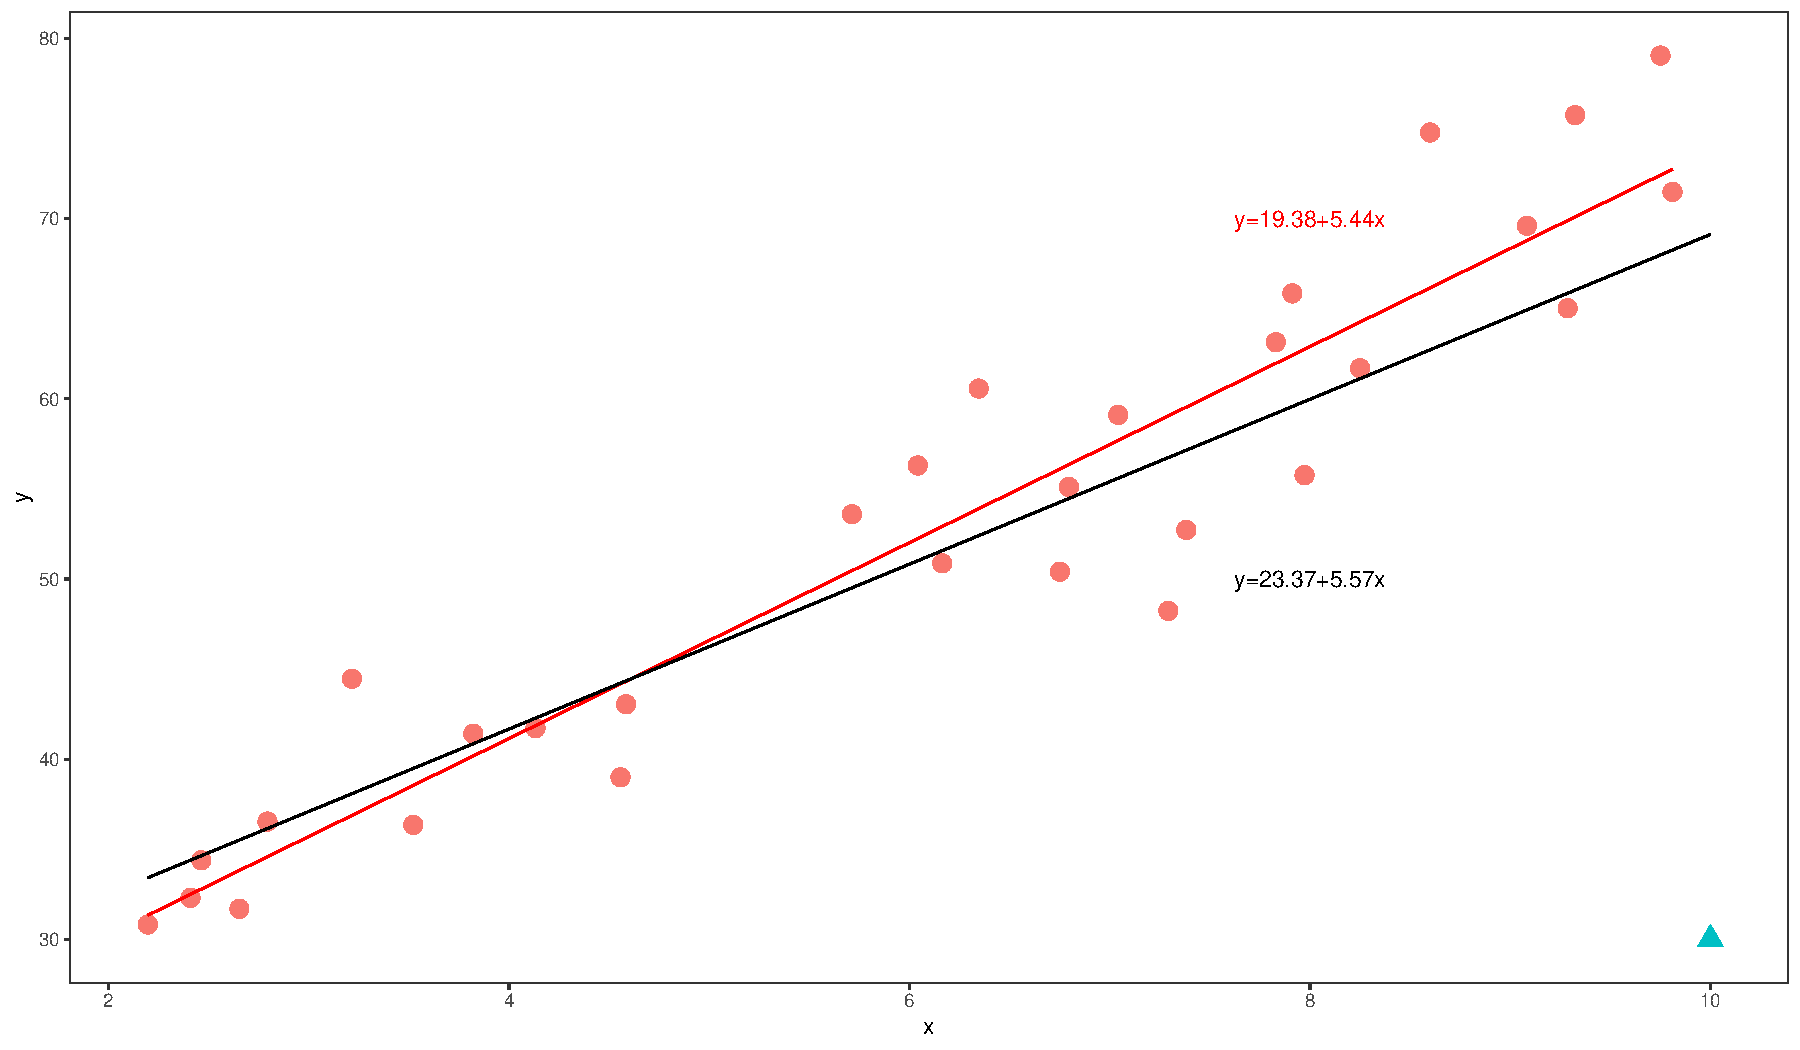
\includegraphics[scale=0.35]{figures/fig_1.pdf}
  \\
  \tiny
\end{figure}


\end{frame}

%----------------------------------------------------------------------%
\begin{frame}
\frametitle{Applications: Leverage}

Consider a dummy variable $e_j$ which is an $n-vector$ with element $j$ equal to 1 and the rest is 0. 
Include it as a regressor

\begin{align}
y =X\beta+\alpha e_j +u
\end{align}

using FWL we can do 
\begin{align}
M_{e_j} y =M_{e_j} X\beta + r
\end{align}

\begin{itemize}
  \footnotesize
\item $\beta$ and {\it residuals} from both regressions are identical
\item Same estimates as those that would be obtained if we deleted observation $j$ from the sample. We are going to denote this as $\beta^{(j)}$
\end{itemize}

Note: 
\begin{itemize}
\item $M_{e_j}=I-e_j(e_j'e_j)^{-1}e_j'$
\item  $M_{e_j} y = y-e_j(e_j'e_j)^{-1}e_j' y= y-y_je_j$
\item  $M_{e_j} X$ is X with the {\it j row } replaced by zeros
\end{itemize}


\end{frame}


%----------------------------------------------------------------------%
\begin{frame}
\frametitle{Applications: Leverage}
Let's define a new matrix $Z=[X,e_j]$
\begin{align}
y &= X\beta+\alpha e_j +u \\
y &= Z\theta +u
\end{align}

then the fitted values 

\begin{align}
y &= P_Z y + M_zy  \\
&= X\hat \beta^{(j)} + \hat \alpha e_j + M_Z y
\end{align}

Pre-multiply by $P_X$ (remember $M_Z P_X=0$) 

\begin{align}
P_X y &= X\hat \beta^{(j)} + \hat \alpha P_X e_j \\
X \hat \beta  &= X\hat \beta^{(j)} + \hat \alpha P_X e_j \\
X (\hat \beta  -  \beta^{(j)} )&= \hat \alpha P_X e_j 
\end{align}
\end{frame}

%----------------------------------------------------------------------%
\begin{frame}
\frametitle{Applications: Leverage}
How to calculate $\alpha$? FWL once again

\begin{align}
M_X y =\hat\alpha M_X e_j + res
\end{align}

\begin{align}
\hat\alpha = (e_j'M_X e_j)^{-1}  e_j'M_X y  
\end{align}

\begin{itemize}
\item $e_j'M_X y $ is the $j$ element of $M_Xy$ is the vector of residuals from the regression including all observations
\item $e_j'M_xe_j$ is just a scalar, the diagonal element of $M_X$

Then 

\begin{align}
\hat\alpha = \frac{\hat u_j}{1-h_j}
\end{align}
\end{itemize}

where $h_j$ is the $j$ diagonal element of $P_X$


\end{frame}
%----------------------------------------------------------------------%
\begin{frame}
\frametitle{Applications: Leverage}
Finally we get 

\begin{align}
  (\hat \beta^{(j)} - \hat \beta)&= - \frac{1}{1-h_j} (X'X)^{-1}X_j'\hat u_j
\end{align}

Influence depends on two factors
\begin{itemize}
  \item $\hat u_j$ large residual $\rightarrow$ related to y coordinate
  \item $\hat h_j$ related to x coordinate $\rightarrow$ if $h_j$ is large, we have a high leverage
\end{itemize}

\begin{figure}[H] \centering
  \centering
  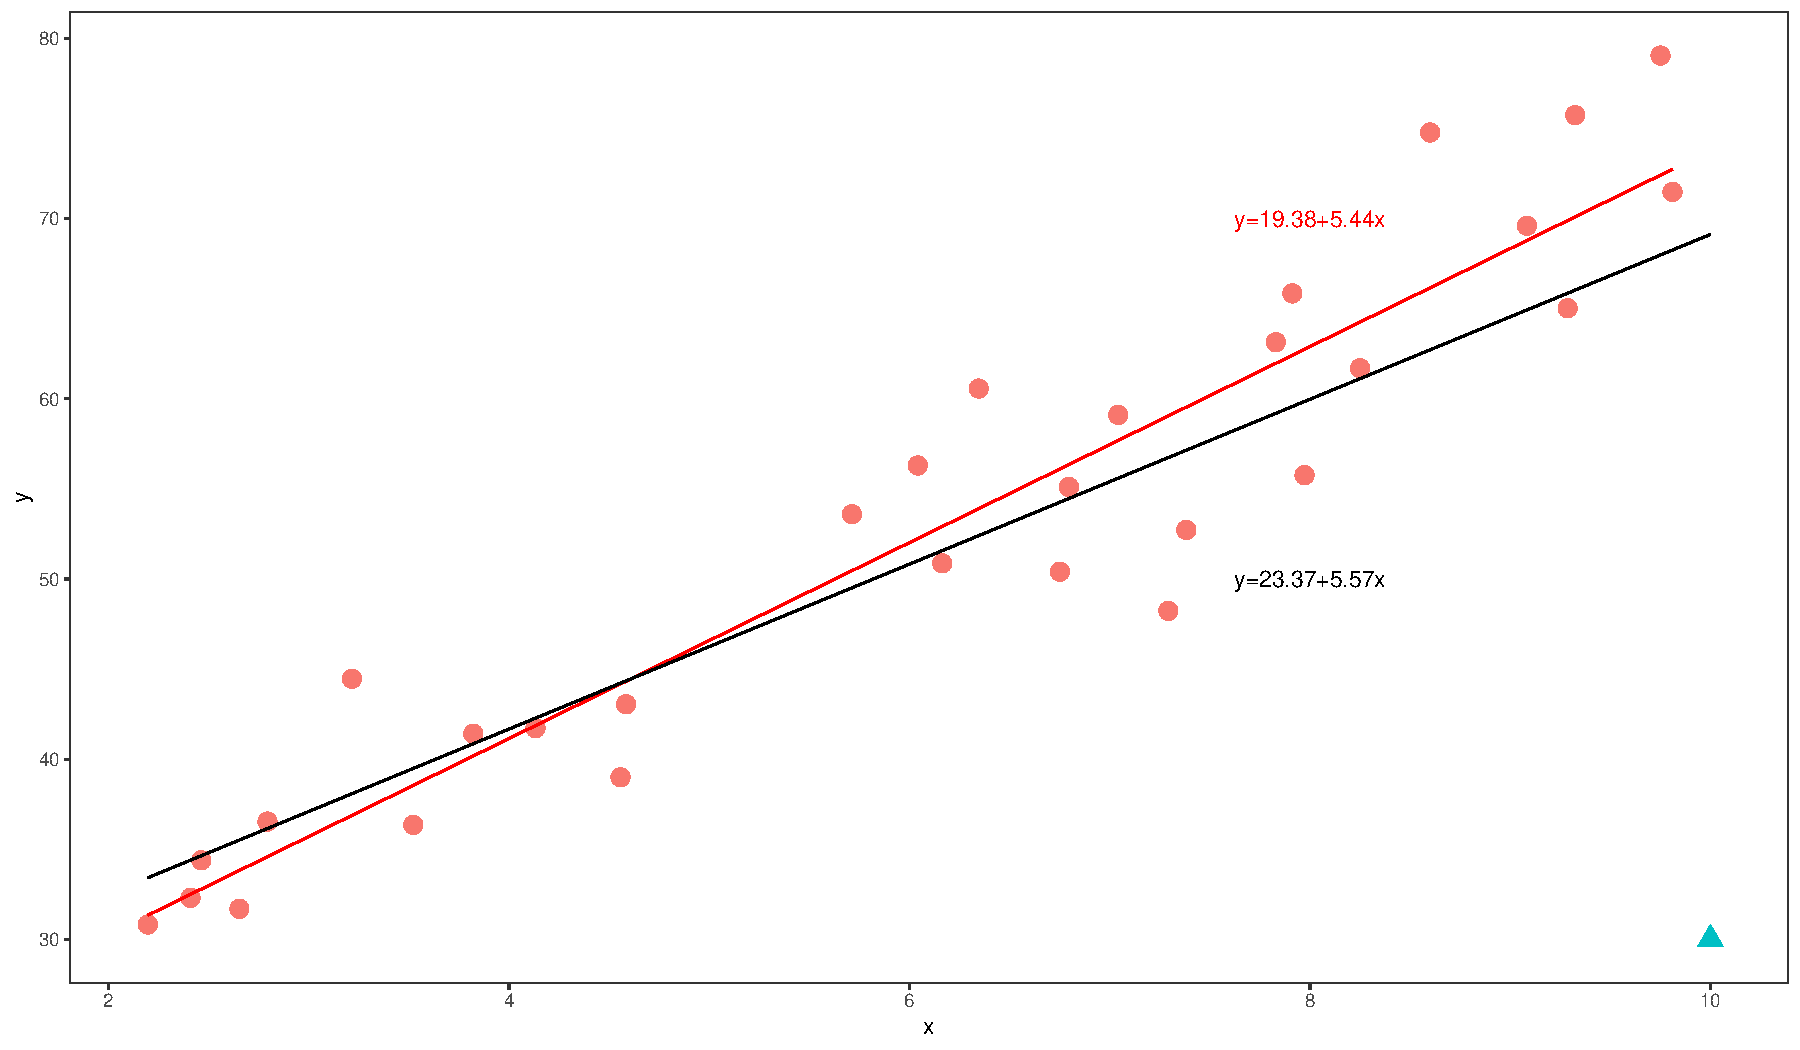
\includegraphics[scale=0.15]{figures/fig_1.pdf}
  \\
  \tiny
\end{figure}
\end{frame}


%----------------------------------------------------------------------%
\begin{frame}
\frametitle{Applications: Leverage}
Case of $y=\alpha + \beta x +u$ (ISLR)

\begin{align}
h_j&=e'_j P_X e_j \\
&. \\
 \text{{\tiny (steps as HW)}}  \\
 &. \\
h_j&= \frac{1}{n}+\frac{(x_j-\bar x)^2}{\sum_{i'=1}^n(x_{i'}-\bar x)^2}
\end{align}


\begin{itemize}
\item Then $h_j$ is always between $\frac{1}{n}$ and 1
\item The average $\sum_j h_j/n$ is always equal to $(k+1)/n$
\end{itemize}


\end{frame}


%----------------------------------------------------------------------%
\begin{frame}
\frametitle{Goodness of Fit}
{\bf $R^2$}: the fraction of the variation of the dependent variable that is attributable to the variation in the explanatory variables
\bigskip
\begin{align}
R^2 = \frac{ESS}{TSS}=\frac{||P_Xy||^2}{||y||^2}=1-\frac{||M_Xy||^2}{||y||^2}
\end{align}

\begin{itemize}
  \item Problem:  not invariant to changes in units, can be negative
  \item In practice we use the centered version:
\end{itemize}

\begin{align}
R^2_c=\frac{||P_XM_\iota y||^2}{||M_\iota y||^2}
\end{align}

{\bf $R^2_c$}: is a measure of the explanatory power of the nonconstant regressors.


\end{frame}
%----------------------------------------------------------------------%
%----------------------------------------------------------------------%
\begin{frame}
\frametitle{Review \& Next Steps}
  
  \begin{itemize} 
    \item What is Big Data?
    \medskip
    \item Quick Review of Statistical Properties
    \medskip
    \item Numerical Properties
    \medskip
    \item FWL
    \begin{itemize}
    \item Fixed Effects
    \item Leverage
    \item Goodness of Fit
  \end{itemize}
  \bigskip  

  
  \item  {\bf Next Class:} OLS Computation, Scraping Data
  \bigskip
  \item Questions? Questions about software? 
  
  \end{itemize}


\end{frame}
%----------------------------------------------------------------------%

\section{Further Readings}
%----------------------------------------------------------------------%
\begin{frame}
\frametitle{Further Readings}
\footnotesize
\begin{itemize}
  \item Carneiro, A., Guimarães, P., \& Portugal, P. (2012). Real Wages and the Business Cycle: Accounting for Worker, Firm, and Job Title Heterogeneity. American Economic Journal: Macroeconomics, 4 (2): 133-52. 
  \medskip
  \item Davidson, R., \& MacKinnon, J. G. (2004). Econometric theory and methods (Vol. 5). New York: Oxford University Press.
  \medskip
  \item Friedman, J., Hastie, T., \& Tibshirani, R. (2001). The elements of statistical learning (Vol. 1, No. 10). New York: Springer series in statistics.
  \medskip
  \item Greene, W. H. (2003). Econometric analysis fifth edition. New Yersey: Prentice Hall.
  \medskip
  \item James, G., Witten, D., Hastie, T., \& Tibshirani, R. (2013). An introduction to statistical learning (Vol. 112, p. 18). New York: springer.
  \medskip
  \item Ruud, P. A. (2000). An introduction to classical econometric theory. OUP Catalogue
  \medskip
  \item Taddy, M. (2019). Business data science: Combining machine learning and economics to optimize, automate, and accelerate business decisions. McGraw Hill Professional.


\end{itemize}

\end{frame}


\end{document}


